\documentclass[12pt]{article}
\usepackage{verbatim}
\usepackage[dvips]{epsfig}
\usepackage{color}
\usepackage{url}
\usepackage[colorlinks=true]{hyperref}

\begin{document}

\section*{GENESIS: Documentation}

{\bf Related Documentation:}
% start: userdocs-tag-replace-items related-workflow
% end: userdocs-tag-replace-items related-workflow

\section*{Developer Workflow Overview}

The typical developer workflow within GENESIS has six basic steps, as the following figure illustrates:
 \begin{figure}[h]
    \centering
    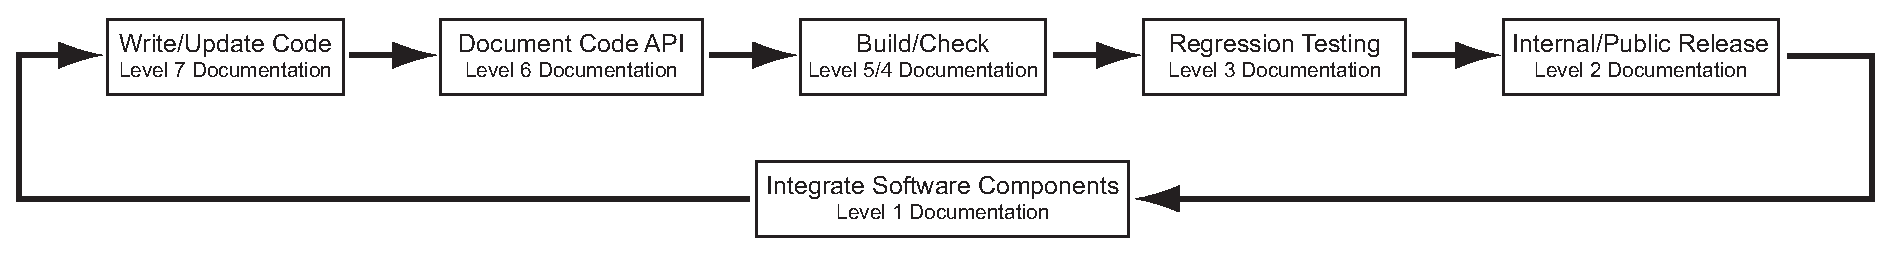
\includegraphics[scale=0.5]{figures/workflow-developer.eps}
    \label{fig:df-1}
 \end{figure}

This figure illustrates the relationship between the developer workflow and the \href{../workflow-user/workflow-user.tex}{\bf User\,Workflow}. It has similarities with the waterfall model of software engineering. It is notable that, with the exception of regression testing, the five steps of the user workflow map directly to the elements of the developer workflow.

The following figure provides a functional view of the developer workflow.
 \begin{figure}[h]
    \centering
    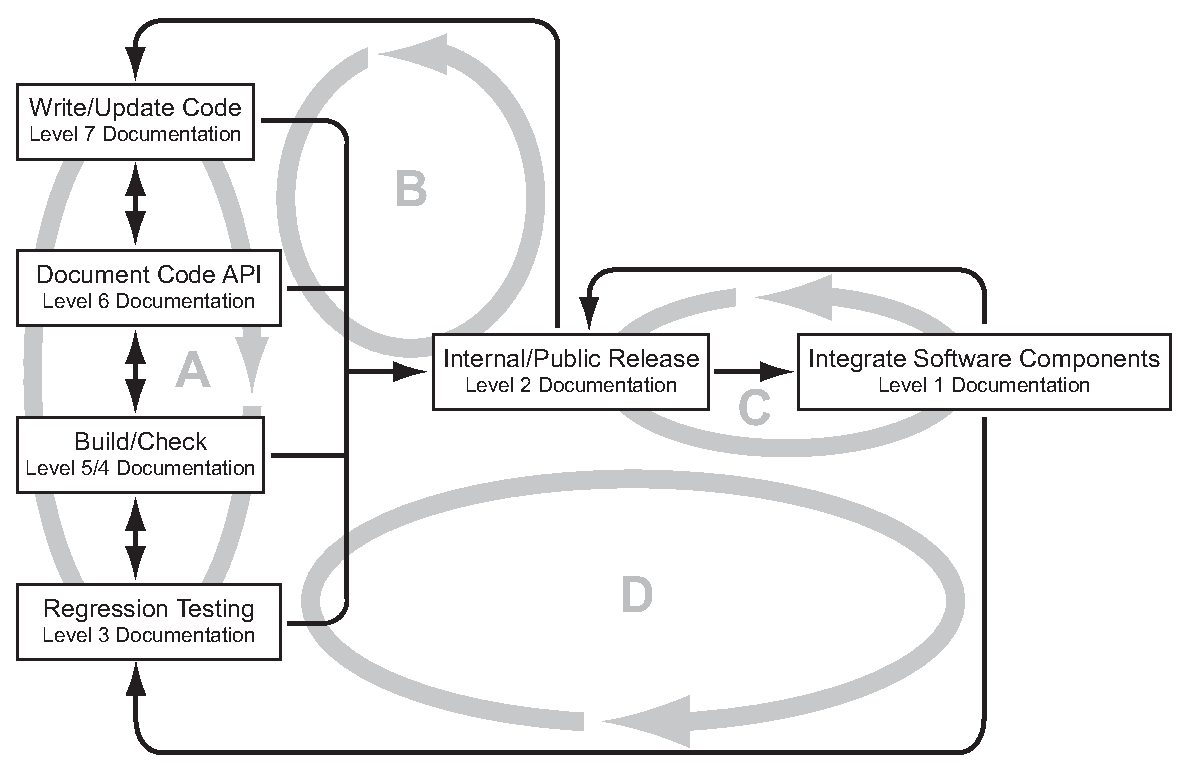
\includegraphics[scale=0.6]{figures/workflow-developer-functional.eps}
    \label{fig:df-1}
 \end{figure}

Importantly, this view of the workflow organizes the developer experience of GENESIS. In doing so, it reveals four interlinked development cycles that lead to the release of a new version of a \href{../reserved-words/reserved-words.tex}{\bf GENESIS component}:
\begin{itemize}
   \item[A.]{\bf Core Development Cycle:} The core development cycle comprises the four fundamental steps required for the development or updating of a software component that complies with the \href{../genesis-overview/genesis-overview.tex}{\bf CBI\,federated\,software\,architecture}. As illustrated in the figure above the steps in this cycle are: Write/Update Code, Document Code API, Build/Check, and Regression Testing.
   \item[B.]{\bf Release Preparation Cycle:} The release preparation cycle adds either an internal and/or public software release to the core development cycle.
   \item[C.]{\bf Release Integration Cycle:} The release integration cycle is comprised of an internal and/or public release associated with the integration of the new component into the GENESIS software platform.
   \item[D.]{\bf Developers Workflow:} The six steps (A--D) comprise the GENESIS developers workflow.
\end{itemize}

As illustrated, the six steps of the developer workflow include:
\begin{enumerate}
\item{\bf Write/Update Code:} The developer workflow starts with the Core Development Cycle (A). This begins with either the writing of code for a new GENESIS component or the updating of a pre-existing software component.
\item{\bf Document Code API:} Essential to the CBI federated software paradigm are the code API's for the interfacing of a new software component with pre-existing GENESIS software. Developers are responsible for the development and documentation of the code API's including source documentation and making them available as Level 6 documentation in the GENESIS Documentation System. This documentation is typically generated by Doxygen or a similar documentation extraction system and is focused on how to interface to the specific implementations of low-level algorithms. 
\item{\bf Build/Check:}
\item{\bf Regression Testing:} Developers are responsible for the development and documentation of regression tests. These provide common use cases and examples of workflows and bridge between the functions visible to a user and the way those functions are implemented in the code. As Level 3 documentation, regression tests also guide developers through the code and define a framework for communication between users and developers. Currently, this level of documentation is automatically generated from test cases. This step of the developers workflow completes the Core Development Cycle (A).
\item{\bf Internal/Public Release:} Prior to an internal release, developers are responsible for providing in-depth Level 2 documentation about the specific functions of a new GENESIS component. This step in the developers workflow extends the Core Development Cycle (A) into the Release Preparation Cycle (B). Completion of the Release Preparation Cycle leads to a public release when a new software component and its associated documentation are pushed to the GENESIS repositories.
\item{\bf Integrate Software Components:} The final step of the Developers Workflow (D) completes the software development cycle. It ensures that a new software component integrates correctly with the pre-existing GENESIS software platform. This step also entails the writing of Level 1 introductory documentation.
\end{enumerate}

\end{document}
